\chapter{Discussion}
This chapter servers to discuss the developed solutions and the results from different aspects. Problems, which occured during the bachlor thesis, are presented as well.

To draw a cell as sphere out of voxels is one way to get the desired spherish shape of the cell. Sadly to keep the shape of the cell during the growth process does not work. Since for a given volume and a given surface there are all kinds of shapes \ac{CC3D} does not know which shape the cell should have. It it suprising that every time the cells get a cubish form during the growth process. It might be a result of the square lattice, which is used in the simulation. There are several research papers, which use \ac{CC3D} for their simulation, sadly it is never explained how the desired cell form is achieved neither which lattice type is used. So far, it is not possible to know if there is an mistake in the simulation or if the cells get a cubish form due to the square lattice. \newline
It is possible that a cell reaches a desired volume and surface, by only setting the terms for the volume and surface of the effective energy. The desired values can be reached faster if a high multiplier, $\lambda_{vol}$ and $\lambda_{sur}$, is set. This has the disadvantage that a volume or an surface constraint might weigh more than the term of the adhesion in the effective energy. If the specific multiplier has a small value, it might be possible that it takes a long time until the desired shape is reached. In addition to the volume and surface constraint comes the adhesion. Adhesion influences the shape of two or more cells, as it describes how strong the stick to each other. If the adhesion is set too high the cells infiltrate each other but if it is too low the cells may not stick to each other as they change their shape. During the simulations it was observable that some cells of different cell types want to infiltrate each other. This is a result of to high adhesion. Which adhesion values has which effects is not explained in the literature. This might be a result that it is possible to simulte a lot of different cell types, which may have different behavior at different adhesion values. Since there is no literature about the adhesion of cells by using \ac{CC3D} it has to be tried out during the simulations. To find the correct adhesion values between cell types has a huge effect on the simulation. Therefore, it might is the only chance to find the correct values, for the desired behavior of the simulation, by trying different adhesion values in different simulation runs. For further research it is important that informations like the adhesion values or about the shape of a cell are shared. It could be result that the published papers are constrained in the length.

In the simulations the voxel density should be set to 1. In this case, in \ac{CC3D}, one \SI{1}{\micro\metre} is presented by one voxel. If the voxel density is higher than one voxel represents less \SI{}{\micro\metre}. Since the simulations requires a lot of more time if the voxel density is higher and the deviation between the volume and surface values of a cell as a sphere out of voxels and a real sphere is larger it should be tried to keep to voxel density as small as possible but also not to small. Why the deviation of a cell and a real sphere grows so much more for a higher voxel density is a puzzle. On one hand the deviation grows with the radius, with more voxels. Since with a higher voxel density there are also more voxels to display it might is a result that \ac{CC3D} uses more voxels to display the cell. On the other hand the volume and surface values of the drawn cell are that high that for the surface of a real sphere a factor of 6 would give an approximation to the surface of the drawn cell. \newline
As it is displayed in figure \ref{img:DeviationSphereCellRealSphere-vD2} the volume of a real sphere and of a drawn sphere cell in \ac{CC3D}, drawn in a simulation with a voxel density of 2, is way to far apart as this voxel density could be used for a realistic simulation of the urothelium. It is interesting to observe that the volume of a sphere cell increases this fast, whereas the surface of a sphere grows in an almost linear way for an increasing radius. Since in \ac{CC3D} in a 3D simulation the volume refers to a physical volume and the surface refers to a physical surface it might be that one voxel still represent \SI{1}{\micro\metre}, even it should be only \SI{0.5}{\micro\metre}. This might explain the results, as they are similiar to the results of $2 \cdot r$ if the voxel densitiy equals 1.
\begin{figure}
	\center
	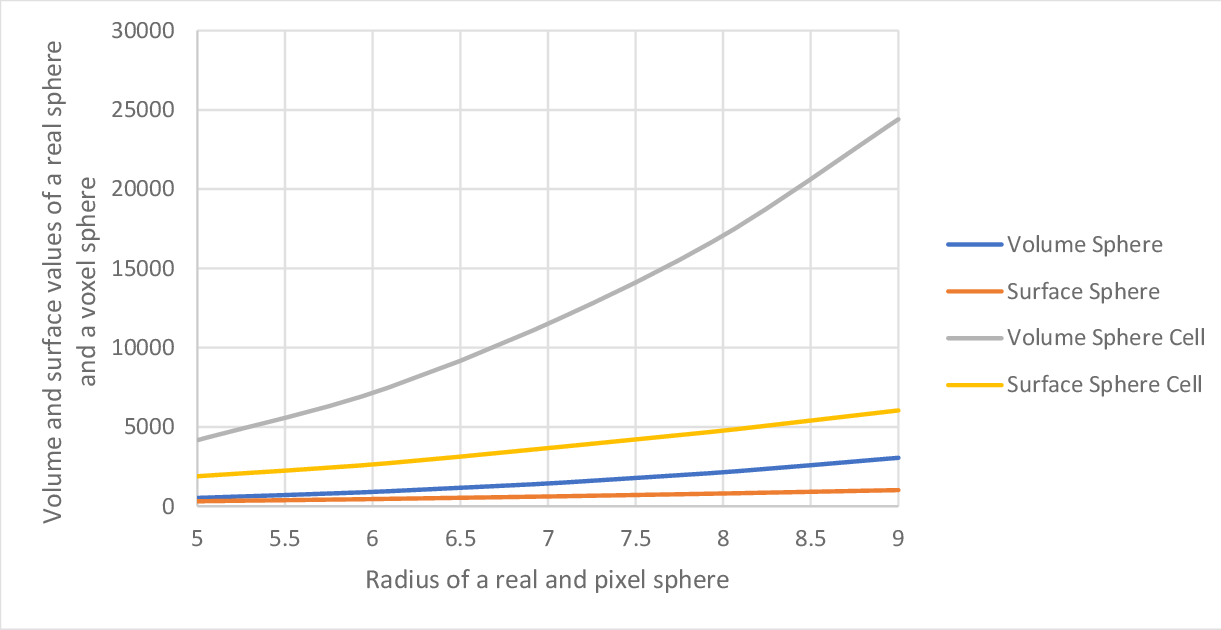
\includegraphics[scale=0.3]{figures/DeviationSphereToPixelSphere-vD2.png}
	\caption{}
	\label{img:DeviationSphereCellRealSphere-vD2}
\end{figure}
%TODO test with vD < 1


The approximation of the surface of a cell to a surface of a real sphere is done with voxels, because these are also used in the simulation field. There are other techniques to approximate the surface of a sphere. It is possible to use pyramids for this approximation. Since in the current simulation the square lattice is used it might is difficult to find an approximation technique which suits the square lattice better. Moreover, the volumes of the cells and of a sphere are almost identical for the same radius. Therefore, the approximation of a cell to the volume of a sphere need also to be checked, since the volume is more important in the simulation as it is listed in table \ref{tbl:CellConstraints} at page \pageref{tbl:CellConstraints}.

\begin{itemize}
\item take a look a biocellion (no race conditions) and morphois
\item use chemical field for growth
\item Random Walker algorithm
\item kugel oberfläche mit pyramiden berechnen (problem wir haben immernoch pixel und square lattice)
\subitem archimedes volumen eines kugelschnittes
\end{itemize}

\section{Calculate Surface Variation Pixels to Sphere}
Two possibilities to design the algorithm
\begin{itemize}
\item check the center of each pixel for the radius, is within the radius or not
\item calculate the y-values of the radius for an x-value of the center of several pixels -> decide dependen on the result of the y-values if the specific pixel is counted or not (if the center of the pixel is within or outside the radius)
\end{itemize}

\section{Approximation \& calculation Errors}
Floating point arithmetic

\section{CC3D}
\begin{itemize}
\item \textbf{CC3D sucks}
\item 400vx $\cdot$ 400vx $\cdot$ 400vx = 107171875vx CC3D has its problem and crashes sometimes on 4GB RAM
\item CC3D does not empty the used RAM after a simulation -> after several simulations the computer will run out of RAM an CC3D crashes
\item no Debug -> testing with print commands at command line
\end{itemize}